\section{ASTRI-Horn data reduction and analysis} 
\label{sect:astridata}

\subsection{Gain evaluation}
\label{subs:gain}

A first step of the data analysis chain is the calibration of the camera pixel gains. 
The ASTRI-Horn camera is equipped with a thermal control system to keep the temperature of the focal plane in a defined range and to monitor it in order to coherently change the voltage applied to the FEE preamplifiers \tem{???} and compensate any following  gain variations. In addition, a dedicated procedure is implemented to improve the level of the gain calibration up to 1\% with an off-line analysis. This method is based on the use of a side emitting fiber optics system (FOC) located along the PMMA window circumference and connected to a controlled intensity diode (LED. It lights almost uniformly the focal plane with an average intensity of a few $p.e.$ per pixel. FOC data are collected periodically during the normal telescope acquisition mode \tem {???}.

FOC data used for this paper data analysis are listed in Table~\ref{tab:FOC}; they are relative to a fixed voltage $V_{0}$= 57 V \tem {di che?} and a temperature of 15$^\circ$C \tem {che vuol dire?}. For these acquisitions HG data are available.

The HG pulse height distribution for both runs listed in Table~\ref{tab:FOC} is accumulated and, for each pixel, the position of the maximum amplitude of each peak is computed fitting the curve with a multi-Gaussian function. Figure~\ref{fig:FOC} shows the pulse height spectrum relative to one of the camera pixel. The gain is computed comparing the average difference between two consecutive peaks centers, $p.e._{eq}$, with that produced by a reference gain $p.e._{ref}$:

\begin{equation}
G_{run ID}\,=\,\frac{p.e._{eq}}{p.e._{ref}}\,G_{ref}
\end{equation}

\noindent
where $G_{run ID}$ is the gain in the considered run, and $G_{ref}$ is the reference one.

\begin{figure*}[ht!!]
\centering
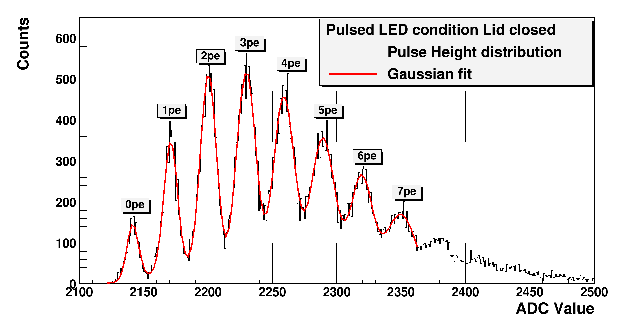
\includegraphics[angle=0, width=12.5cm]{Figure/PIXEL60_PDM20_HG_DICEMBRE_2018.eps}
\vspace{0.5cm}
\caption{ Pulse height spectrum for one of the camera pixel during a FOC acquisition (black curve); data are relative to the HG electronics chain. The red curve shows the multiple peaks Gaussian fit.}
\label{fig:FOC}
\end{figure*}

\begin{table*}[htbp!!]
\centering
\caption{Log of FOC data used in the analysis. For these runs HG data are considered. }
\begin{tabular}{lccc}
\hline\hline
Run ID & Starting Date &  Exposure & Number of events \\
               & (year/month/day h:m:s) & (s)   \\
\hline     
1394 & 2018/12/02 20:01:09  &  & 60065     \\
1763 & 2019/03/23 20:01:21  &  & 120123    \\ 
\hline\hline
\end{tabular}
\label{tab:FOC}
\end{table*}

\subsection{Open sky data} 
\label{subs:skydata}

Background data used for the analysis refer to the period between December 2018 and March 2019 when the telescope was mainly involved in the Crab observation campaign. The list of the considered run ID is reported in Table~\ref{tab:obslog}; runs are split in several files, each containing a maximum of 50000 events, identified with a progressive number.
A selection was applied in order to avoid data affected by technical problems as instability in the PDM signals or fluctuation of the trigger rate. Moreover, intervals with bad atmospheric conditions 
(high humidity, low external temperature, cloudiness) were not considered as well as the periods when UVscope data are not available.

In each detected events we considered only the nine central PDM (11, 12, 13, 18, 19, 20, 25, 26, 27 in Fig.~\ref{fig:camera}) taking into account the smaller UVscope FOV.  In addition, bad pixels and pixels imaging stars with a magnitude higher than …, coherently with the procedure adopted for UVscope data, are excluded from the analysis. The position of the stars in ASTRI-Horn FOV is computed from the correspondence with UVscope pixels derived from the variance method \citep{Segreto2019}. 
The variance method was not used to identify stars because the relative data were not available in December and, for uniformity in the analysis, we decide to not use it either in March.  However, March variance data were used to cross-check the positions obtained from the correspondence with UVscope pixels.

\begin{table}[ht]
\caption{ASTRI-Horn observation log}
\centering
\begin{tabular}{lcccc}
\hline\hline
Run ID & Starting Date & Exposure      & N. of events & pointing \\
               & (year/month/day h:m:s) & (s)  \\
\hline     
%https://www.overleaf.com/project/5e3005eb54e0d8000155a7ff
%\footnote{ Azi$=180°$ EleV. $=70°$}
1429 & 2018/12/05 20:57:37  &   2094     & 31755 & Crab Off    \\
1430 & 2018/12/05 21:54:40  &   909      & 29808 & Fixed AltAzi$^*$    \\
1431 & 2018/12/05 22:22:29  &   3573     & 133190 & Crab     \\ %133188
1432 & 2018/12/05 23:30:12  &   3790     & 450000 & Crab     \\ %449998
1433 & 2018/12/06 01:27:41  &   7638     & 198341 & Crab Off    \\ %198303
1434 & 2018/12/06 03:36:06  &   4499     & 142610 &  Fixed AltAzi$^*$  \\ %142583   \\
1453 & 2018/12/07 20:06:11  &   6016     & 348442 & Crab Off    \\
1454 & 2018/12/07 22:09:16  &   4377     & 226651 &  Crab \\ %226650  \\
1455 & 2018/12/07 23:30:08  &   6243     & 412451 &  Crab \\ %412446    \\
1456 & 2018/12/08 01:24:48  &  8530     & 237318 & Crab Off \\ %  237186 \\
1457 & 2018/12/07 03:50:20  &  3509     & 126295 & Fixed AltAzi$^*$\\ % 126264   \\
1464 & 2018/12/08 20:30:37 &  2255 & 97257 & Crab Off \\ %97251 \\  
1465 & 2018/12/08 21:17:34 &  9624 & 430245 & Crab\\ % 430222\\  
1466 & 2018/12/09 00:07:25 &  3161 & 251442 & Crab \\ %251418  
1467 & 2018/12/08 01:09:44 &  8959 & 243713 & Crab Off \\ %243399
1468 & 2018/12/08 03:40:11 &  1237 & 33168 &  Fixed AltAzi$^*$\\ %33126
% **the runs 1488_001 and 1488_002 present an error in TELAPSE keyword 
1472 & 2018/12/09 19:55:03 &  4958 & 185142 &  Crab Off \\ % 185120
1473 & 2018/12/09 21:28:40 &  5549 & 266294 &  Crab\\ %266283
1474 & 2018/12/09 23:19:17 &  3508 & 239982 &  Crab \\ %239954
1475 & 2018/12/10 00:43:51 &  396 & 50989 &  Crab Off \\ %50984
1486 & 2018/12/11 23:02:02 &  1627 & 100948 &  Crab\\ %100947
1487 & 2018/12/11 23:31:48 &  4800 & 259447 &  Crab\\ %259443
1488 & 2018/12/12 01:01:45 &  4638+** & 297577 &  Crab Off\\ %297517
1489 & 2018/12/12 03:02:43 &  1744 & 73285 &  Crab Off \\ %73268
1490 & 2018/12/12 03:34:02 &  5705 & 125218 &  Fixed AltAzi$^*$\\ %124197
1658 & 2019/03/05 18:13:58 &  112 & 1435 & Merak \\  
1659 & 2019/03/05 18:19:26 &  154 & 3149 & Zeta Tauri \\  
1660 & 2019/03/05 18:24:37 &  6224  & 419636 & Crab \\ %419631  
1661 & 2019/03/05 20:10:15 &  168 & 14389 & Zeta Tauri \\  
1662 & 2019/03/05 20:19:59 &  4008 & 198186 & Crab Off \\   
1663 & 2019/03/05 21:29:34 &  2337 & 165264 &  Fixed AltAzi$^*$ \\  
1670 & 2019/03/06 18:08:27 &  628    &   8191      &  Merak\\
1671 & 2019/03/05 18:21:51 &  126        &   2412   & Zeta Tauri \\
1672 & 2019/03/05 18:25:56 &  5935    &   296073   &  Crab \\ %296046
1673 & 2019/03/05 20:06:58 &  183      &   3272     & Zeta Tauri\\ %3270
1674 & 2019/03/05 20:13:37 &  13812      &    152393 & Crab Off  \\ %152110     \\
%1466 & 2018/12/09 20:47:50 &  1218 & 50000 \\  
\hline\hline
\multicolumn{5}{l}{$^*$ Azi$=180^\circ$ Elev. $=70^\circ$}
\end{tabular}
\label{tab:obslog}
\end{table}



Background pixels were identified applying the same double cut cleaning procedure used for the Cherenkov shower images. This procedure considers background pixels the ones that have a signal lower than a first threshold $S1$, or , if higher than $S1$, with none of the neighboring pixels with a signal higher that the second threshold $S2$. In our analysis, we adopted the values $S1$=6 and $S2$=12 used by \cite{Mineo2019} instead of higher values adopted for the analysis of Crab events \citep{Lombardi2020} to avoid muon signals.

For each event we then accumulated the distribution of the number of $p.e.$ in the background pixels. The curve obtained for the file 1473 of the run ID 000 is plotted in Fig.~\ref{fig:distr} as example. It is a distribution with a Gaussian shape in the central part and with long wings due to residual signals in the positive part and to \tem {????} in the negative one. 

The central part of the distribution is then fitted with a Gaussian whose $\sigma$ is the measure of the NSB fluctuations that, being a Poisson signal, is linked to the absolute flux. The RMS values for December 9--10 observation night are plotted in Fig.~\ref{fig:rms} as function of time.

Finally, we plot the resulting values of $\sigma$ for each observing night in Fig.\ref{fig:sigma}  as a function of time. 


\subsection{Closed camera data} 

As explained in Sect.~\ref{sect:intro}, the $\sigma$ of the background distribution is obtained by the sum of the intrinsic noise plus the fluctuations due to the NSB flux level. The first component can be obtained by events acquired with the camera lids closed in absence of light.
Observations used for this analysis are listed in Table~\ref{tab:dark}. In this case, data from LG electronics chain are considered and pulse height spectra for each camera pixels are accumulated adding the contributions of the two considered observations. These are mainly composed by a single peak, the pedestal, that is fitted with a Gaussian function whose $\sigma$ is the measurement of $\sigma_{dark}$. As example the distribution relative to one of the camera pixel in the run ID 1616 is plotted in Fig.~\ref{fig:dark}.


\begin{figure*}[h!!]
\centering
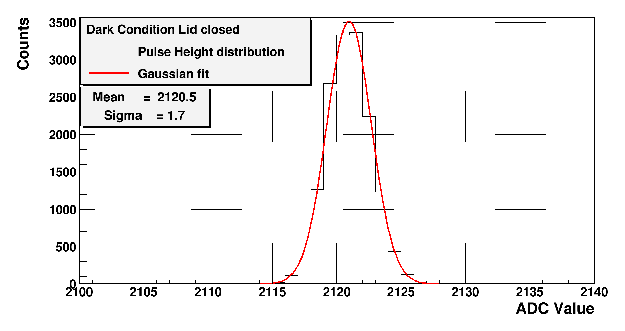
\includegraphics[angle=0, width=12cm]{Figure/PIXEL60_PDM20_LG_DICEMBRE_2018.eps}
\vspace{0.5cm}
\caption{ Pulsed height distribution in one of the camera pixel relative to the runs listed in
Table~\ref{table2} (black curve), the the relative fit with a Gaussian (red curve).}
\label{fig:dark}
\end{figure*}
\label{subs:skydata}


\begin{table*}[htbp!!]
\centering
\caption{Log of closed lid observations. For these runs, LG data are considered.}
\label{tab:dark}
\begin{tabular}{lccc}
\hline\hline
Run ID & Starting Date & Exposure     & Number of events \\
               & (year/month/day h:m:s)   \\
\hline     
1380 & 2018/12/01 20:59:18  &       & 15305      \\
1616 & 2019/02/28 12:37:02  &      & 50000     \\
\hline\hline
\end{tabular}
\end{table*}
